
\documentclass[xcolor=dvipsnames,xcolor=table]{beamer} 
%\documentclass[xcolor=table]{beamer}
%\setbeamercolor{structure}{fg=OliveGreen!80!black} 
\setbeamercolor{structure}{fg=blue!35!black} 
\usetheme{Madrid} 
%\usetheme{Frankfurt}
\usefonttheme{professionalfonts}
\setbeamertemplate{footline}[frame number]

\usepackage[utf8]{inputenc}   % Para reconhecer o conjunto de
				% caracteres latin1 (á) na entrada (.tex) e evitar a necessidade
				% de utilizar o formato tradicional: (\'a)
%\usepackage[T1]{fontenc}
\usepackage[portuges,brazil]{babel}
\usepackage{graphicx}           % Para importar figuras
\usepackage{float}		%aaa Para posicionar as figuras de forma mais conveniente
\usepackage{url}		%aaaa Para imprimir corretamente URLs
\usepackage{enumerate}		%aaaa Para poder enumerar com letras ao inves de numeros
\usepackage{amsmath}
\usepackage{amssymb}
\usepackage[amssymb]{SIunits}
\usepackage{epsfig}

%\usepackage{subfig}
%\usepackage{mathtools} %para os box
\usepackage{amsfonts}
\usepackage{multirow}
%\usepackage{subfigure}
\usepackage{array}
\usepackage{dsfont}
\usepackage[ruled,vlined,portuguese]{algorithm2e}

\newcommand{\bydef}{\stackrel{\Delta}{=}}
\usepackage{mathtools}
\usepackage{calc}
\usepackage{xcolor}
\usepackage{tikz}
\usetikzlibrary{calc}
\usepackage{booktabs}
\usepackage{comment}
%\usepackage[table,xcdraw]{xcolor}

\usepackage{psfrag}
\usepackage{lmodern}

\usepackage{color} % Necessario apenas na fase de revisao.
\usepackage{verbatim} % Necessario apenas para comentar o codigo
\usepackage{colortbl}

\usepackage{ragged2e}

\usepackage{listings} % inserir codigos

\newtheorem{hyp}{Hip\'otese} % para facilitar a vida
%\usepackage[morefloats=100]{morefloats} % para poder processar mais figuras: 18+morefloats = maxfloats
\usepackage{icomma} %detecta automaticamente separador decimal com virgula, sem precisar usar 0{,}0, fica apenas 0,0.

\usepackage{amsopn} %para utilizar o \DeclareMathOperator{\"Operador"}{"operador"}, sem aspas claro
\DeclareMathOperator{\Tr}{Tr} % Tr(A): Traço da matriz A
\DeclareMathOperator{\He}{He} % He{A} = A+A', hermitiano da matriz A.
\DeclareMathOperator{\pol}{pol} % pol: polinomio



\usetikzlibrary{shapes,arrows,positioning}

\tikzset{decision/.style={diamond, draw, fill=blue!20, text width=4.5em, text badly centered, inner sep=0pt}}
\tikzset{block/.style={rectangle, draw, fill=blue!20, text width=5em, text centered, rounded corners, minimum width=3.5cm}}
\tikzset{line/.style={draw, -latex}}




\mode<presentation>



%  \setbeamertemplate{blocks}[rounded][shadow=true]
%\setbeamertemplate{itemize subitem}{$\diamond$}

\title[Eldorado]{Proposta de solução para o desafio Eldorado.}
\author[prof.israel@gmail.com]{Israel Gon{\c c}alves de Oliveira}
\institute[Processo seletivo]{Instituto de Pesquisas Eldorado \\  Parque Científico e Tecnológico da PUCRS}

\date{Porto Alegre, fevereiro de 2018.}

% put color to \boxed math command
\newcommand*{\boxcolor}{orange}
\makeatletter
\renewcommand{\boxed}[1]{\textcolor{\boxcolor}{%
\tikz[baseline={([yshift=-1ex]current bounding box.center)}] \node [rectangle, minimum width=1ex,rounded corners,draw] {\normalcolor\m@th$\displaystyle#1$};}}
 \makeatother

% colrir celula


\newcommand{\Sum}{\sum\limits}
\newcommand{\Lim}{\lim\limits}
% variaveis


\begin{document}


\begin{frame}
\titlepage
\end{frame}

\begin{frame}\frametitle{Contents}
{\footnotesize \tableofcontents}
\end{frame}



\section{Introdução}
\begin{frame}\frametitle{Introdução}

\begin{itemize}
\item Base de dados no formato CSV, contendo 21.120 amostras com 24 características (\emph{features}), sendo a primeira o alvo (\emph{target}), a segunda a hora, seguida de mês e ano, a terceira e quarta, respectivamente. As demais 20 são variáveis não caracterizada (ou, nenhuma informação a priori). Todos as características são números, algumas amostras com informação faltante, nomeado com 'NA'.
\item Objetivo: "realizar a previsão do Target para todos os meses de 2018 e para o
ano de 2018".
\item Com uma análise visual com evidências no domínio frequencial e com base nos histogramas, optou-se por utilizar apenas os valores de alvo e temporais de mês e ano. A solução proposta é baseada na esperança matemática, ou seja, usado o valor médio.
\item A aplicação para análise e solução foi desenvolvida em MATLAB \cite{MATLAB:2014} rodando no GNU/Linux Ubuntu 16.04.3 LTS.
\end{itemize}

\end{frame}


\section{Análise}

\subsection{Pré-formatação}
\begin{frame}[fragile]\frametitle{Análise: pré-formatação.}

\begin{itemize}
\item Os dados foram disponibilizados no formato CSV, arquivo texto. Como os valores usavam vírgula com separador decimal, foi necessário uma substituição para o ponto, para que fosse lido corretamente (não apenas pelo MATLAB, mas para outros softwares testados).

\item Os valores faltantes continham os caracteres 'NA', e foram substituídos por 'nan', para que o MATLAB lesse como um valor não numérico (NaN: \emph{Not a Number}).

\item Código utilizado:

\lstset{numberstyle=\small, numbersep=4pt, frame = single, language=bash}
\begin{lstlisting}
 $ cat data.csv |sed -e 's/\,/\./g' \
     |sed -e 's/NA/nan/g' >data_mod.csv
\end{lstlisting}
\item Para tal processo poderia se usar um editor de texto, visto que o arquivo da base tinha tamanho de 5 MB, todavia isso seria inviável para arquivos muito maiores.

\end{itemize}
\end{frame}

\begin{frame}[fragile]\frametitle{Análise: pré-formatação.}

\begin{itemize}
\item Para as amostras com informação faltante apenas no mês e ano, foi realizada uma substituição do valor 'nan' pelo valor da amostra anterior. Esse processo contempla a grande maioria das amostras com 'NA' nos campos mês e ano de forma correta, visto que as amostras estavam em sequência temporal. Avaliou-se que o ganho de amostras válidas para uso traria um incremento de informação relevante com o custo de raras as amostras com valor possivelmente errado e mês e ano em uma unidade. Não foram aproveitadas as amostras com 'NA' no campo alvo.

\item De um total de 21.120 amostras, foram aproveitadas 18.870, perdendo 2.250 (representando 10,6\% da base original). Das amostras aproveitadas, 1.895 tiveram o ajuste no campo mês e 1.792 no campo ano, representando 10\% e 9,5\% das amostras aproveitadas, respectivamente.

\end{itemize}
\end{frame}


\subsection{Visualização}
\begin{frame}\frametitle{Análise: visualização}

\begin{itemize}
\item Verificar a média, desvio padrão, máximo e mínimo mensal.
\item Verificar a relação mensal e anual.
\item Sem um padrão anual significativo.
\item No gráfico dos valores mínimos há um padrão mensal aparente.
\item Os anos de 2012 e 2013 parecem atípicos e os últimos dois anos apresentam uma queda contínua. Todavia, um padrão é identificado entre esses pares: o ano anterior se mostra como tendência.
\end{itemize}
\end{frame}

\begin{frame}\frametitle{Análise: visualização}
\begin{figure}[htpb] \begin{center} 
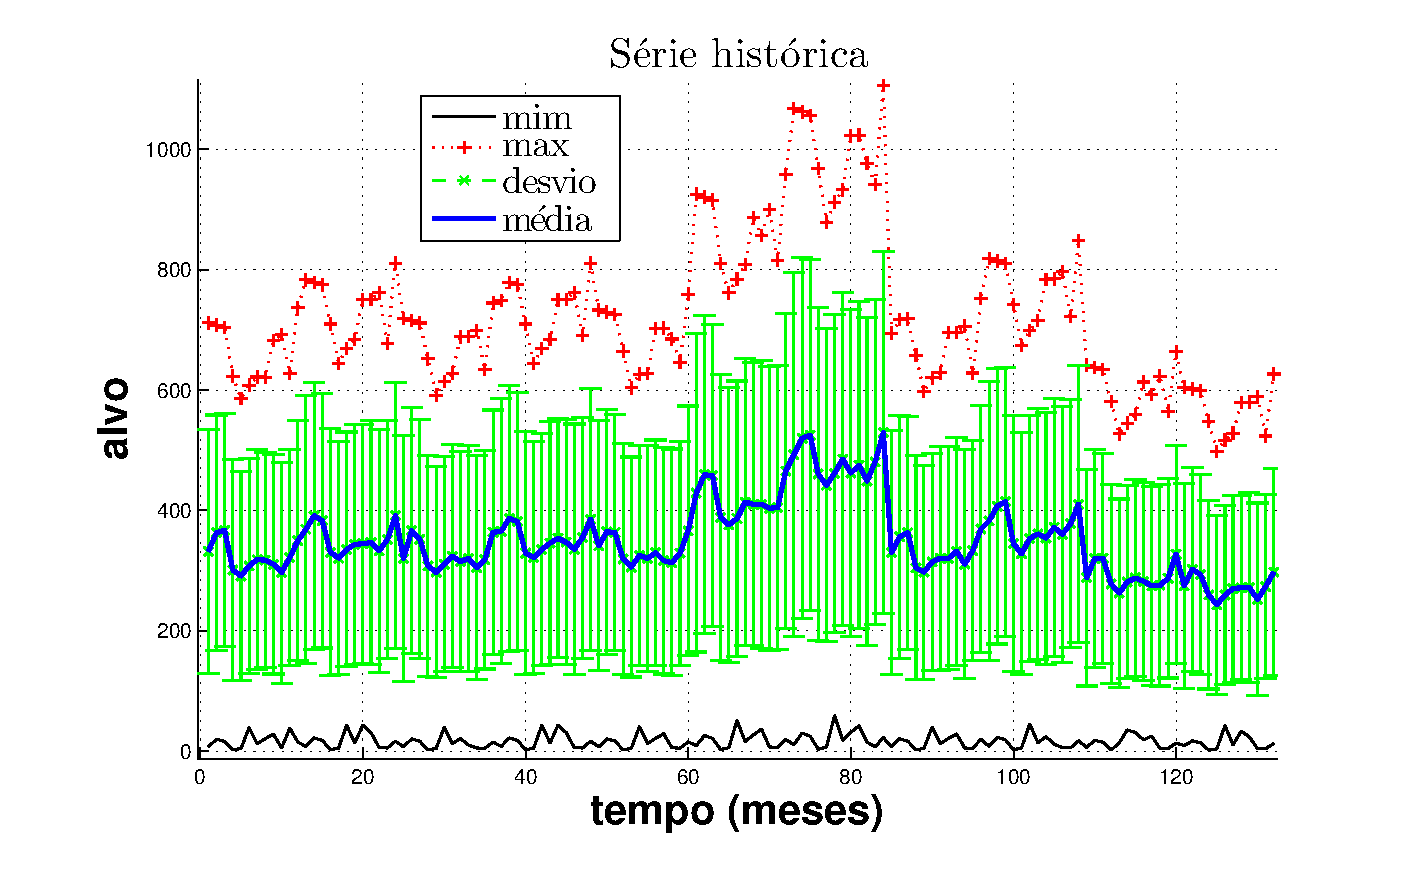
\includegraphics[width=0.9\columnwidth]{seriehist}
\end{center}
\end{figure}
\end{frame}


\begin{frame}\frametitle{Análise: visualização}
\begin{figure}[htpb] \begin{center} 
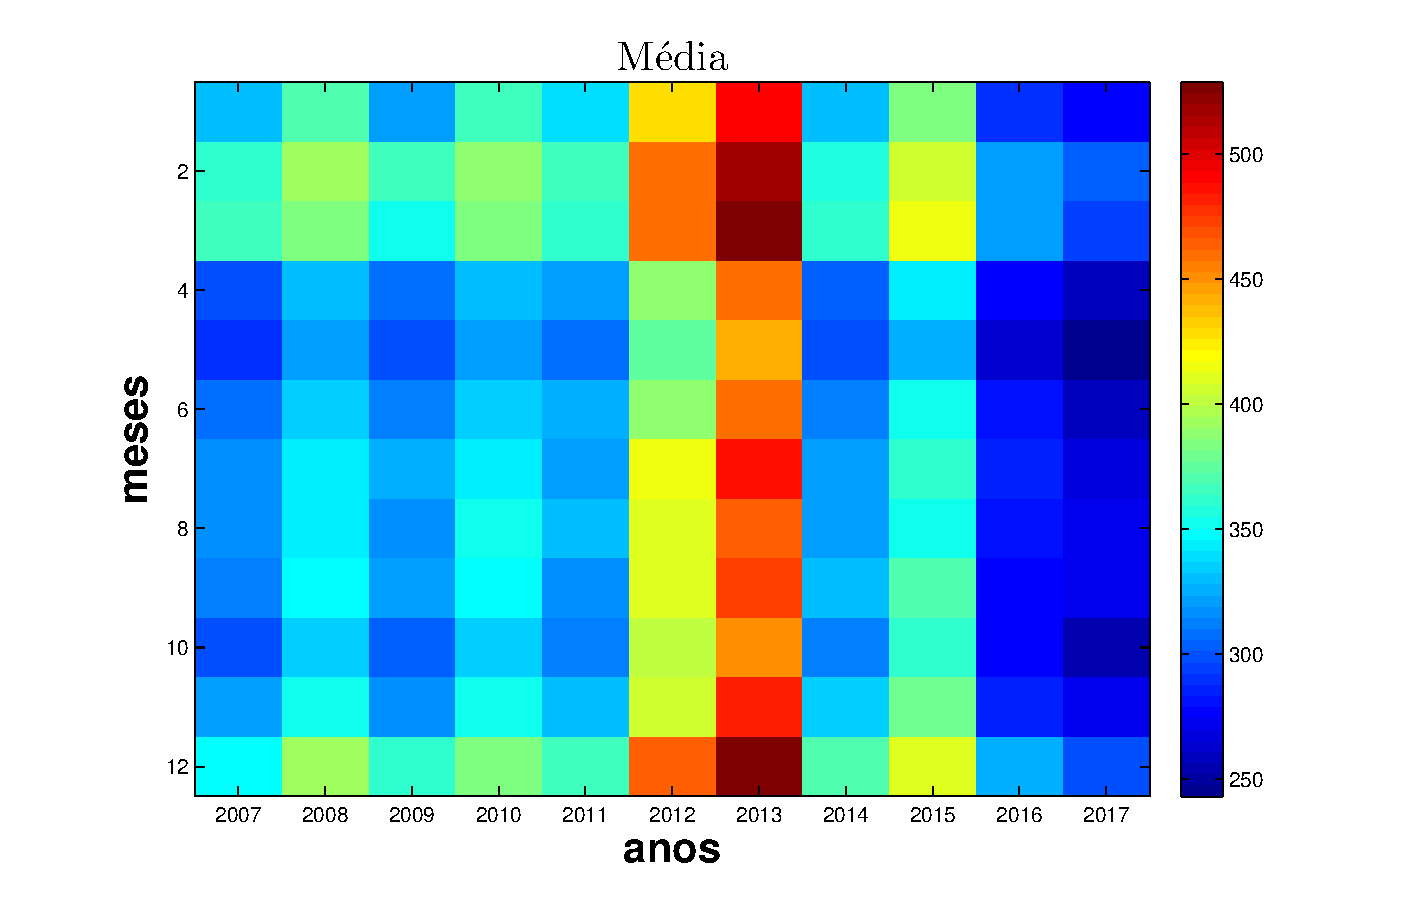
\includegraphics[width=0.9\columnwidth]{media1}
\end{center}
\end{figure}
\end{frame}

\begin{frame}\frametitle{Análise: visualização}
\begin{figure}[htpb] \begin{center} 
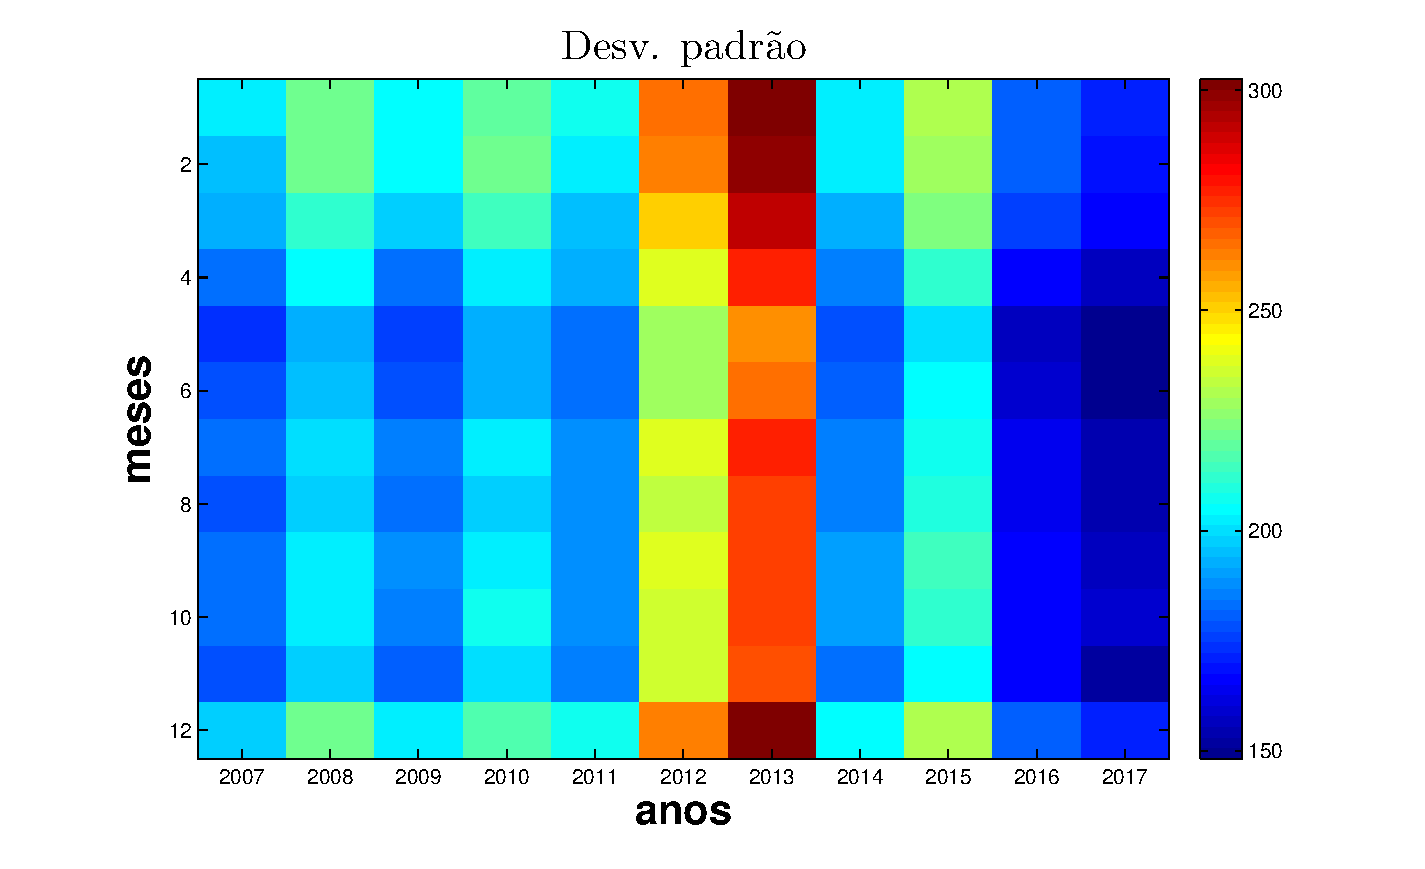
\includegraphics[width=0.9\columnwidth]{sd1}
\end{center}
\end{figure}
\end{frame}

\begin{frame}\frametitle{Análise: visualização}
\begin{figure}[htpb] \begin{center} 
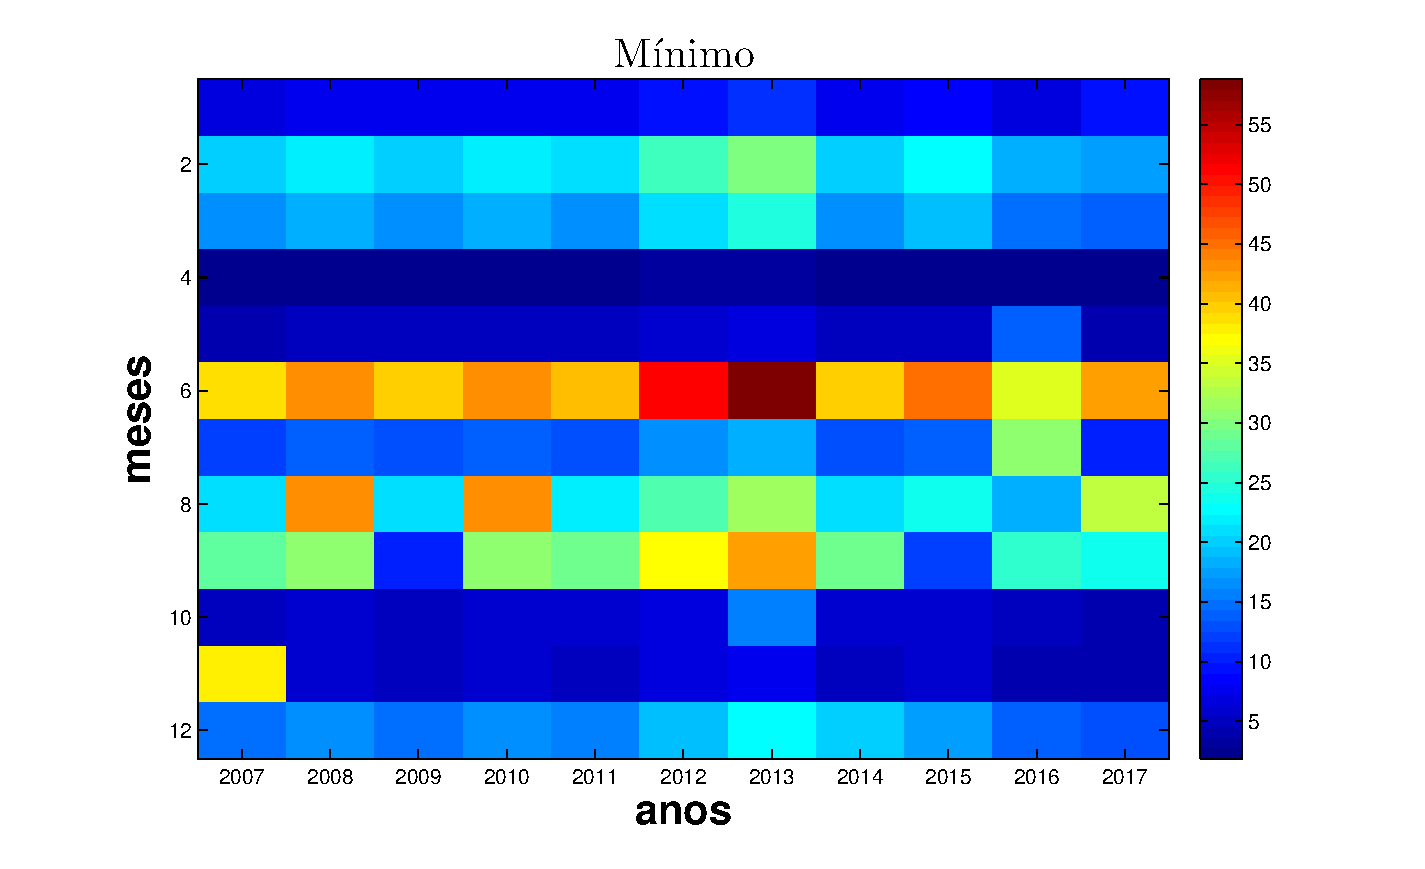
\includegraphics[width=0.9\columnwidth]{min1}
\end{center}
\end{figure}
\end{frame}

\begin{frame}\frametitle{Análise: visualização}
\begin{figure}[htpb] \begin{center} 
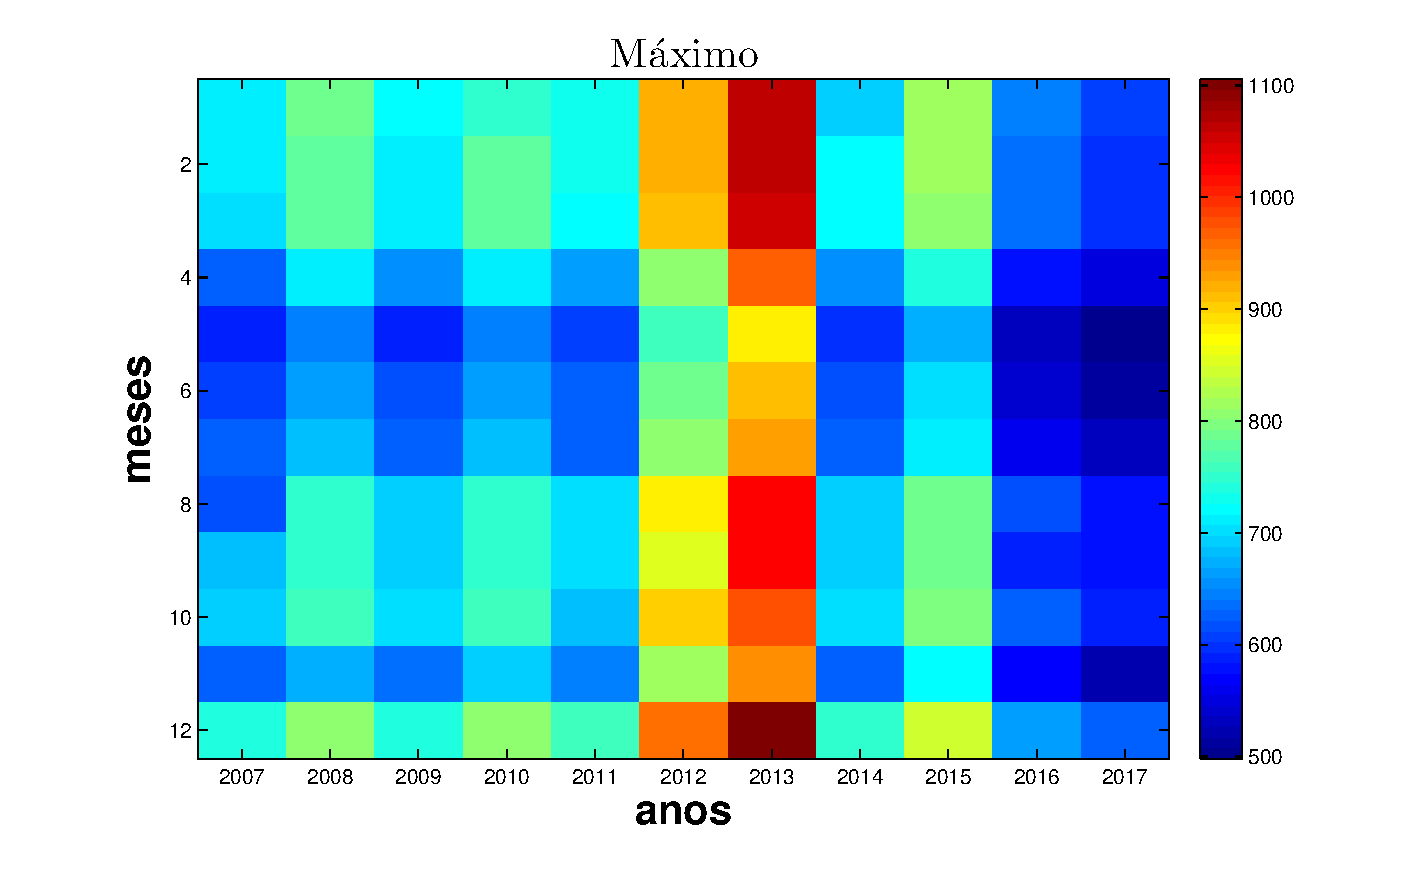
\includegraphics[width=0.9\columnwidth]{max1}
\end{center}
\end{figure}
\end{frame}

\subsection{Visualização no domínio frequencial}
\begin{frame}\frametitle{Análise: Visualização no domínio frequencial}

\begin{itemize}
\item A fim de se obter evidências numéricas quanto aos padrões, pode-se usar uma análise frequencial. O grau de periodicidade de um sinal é relacionado a boa estimativa do sinal utilizando uma expansão de \emph{Fourier}. Não apenas para estimativa mas também pode-se evidenciar o grau de ruído. Um alto desvio padrão pode ser ocasionado pelo ruído.

\item Conforme a análise, a periodicidade mensal é predominante e não há aparente periodicidade anual.

\item Componentes de baixa frequência são dominantes, sugerindo que o uso de valor médio poderia oferecer melhor estimativa.

\end{itemize}

\end{frame}

\begin{frame}\frametitle{Análise: Visualização no domínio frequencial}
\begin{figure}[htpb] \begin{center} 
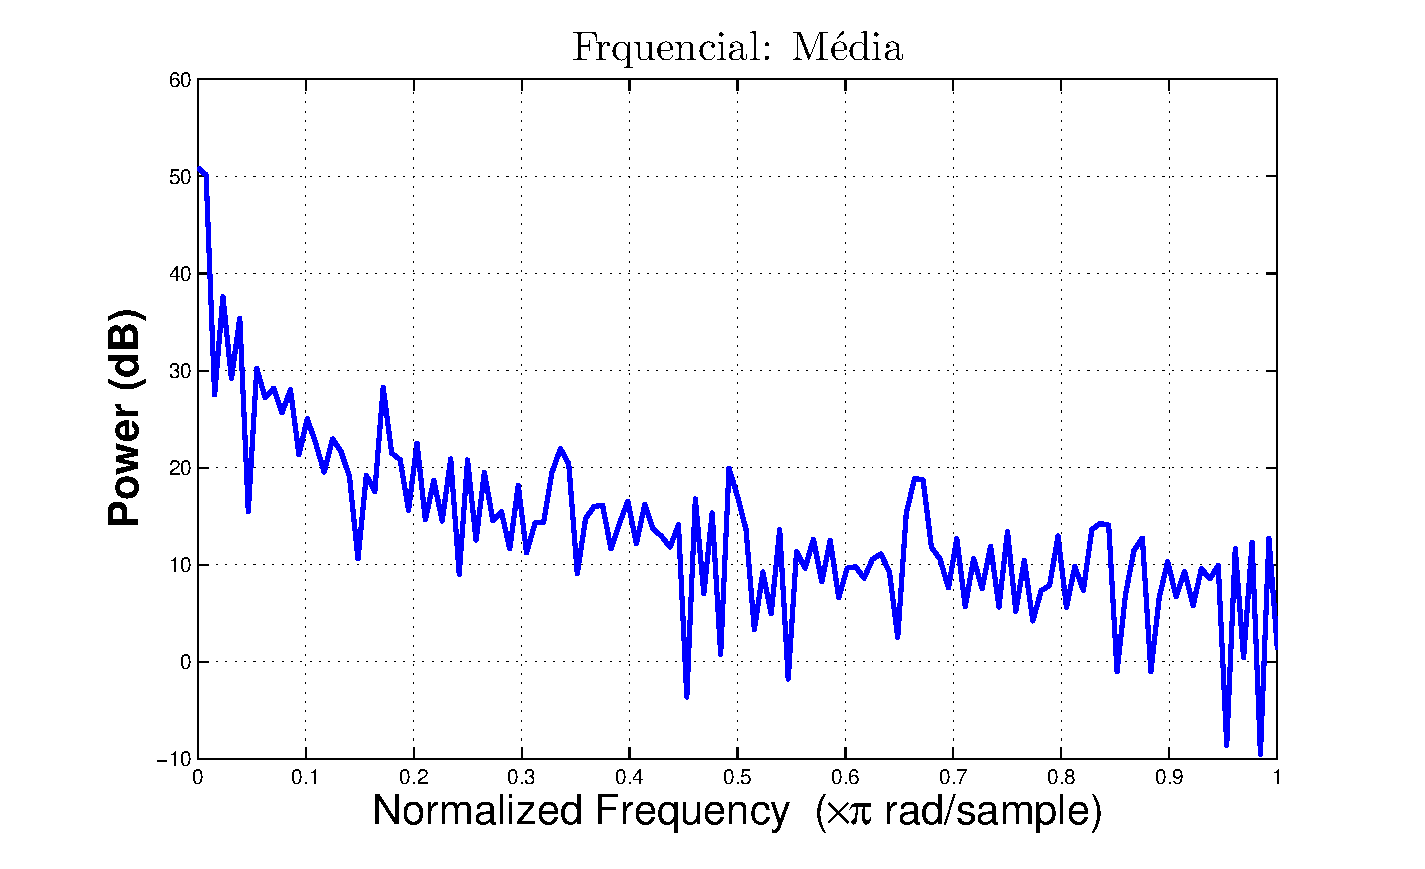
\includegraphics[width=0.9\columnwidth]{fq1}
\end{center}
\end{figure}
\end{frame}

\begin{frame}\frametitle{Análise: Visualização no domínio frequencial}
\begin{figure}[htpb] \begin{center} 
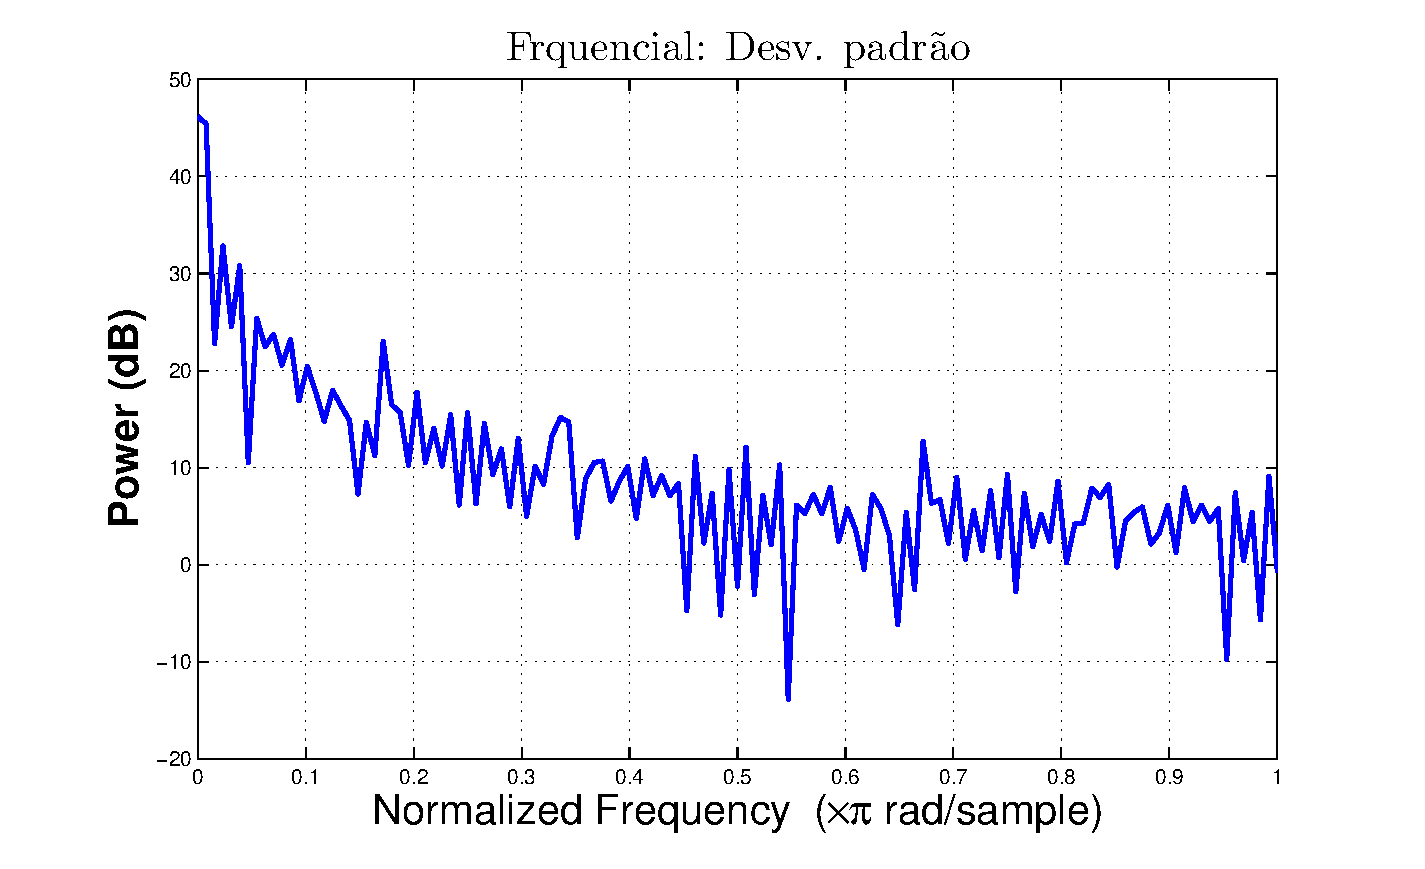
\includegraphics[width=0.9\columnwidth]{fq2}
\end{center}
\end{figure}
\end{frame}

\begin{frame}\frametitle{Análise: Visualização no domínio frequencial}
\begin{figure}[htpb] \begin{center} 
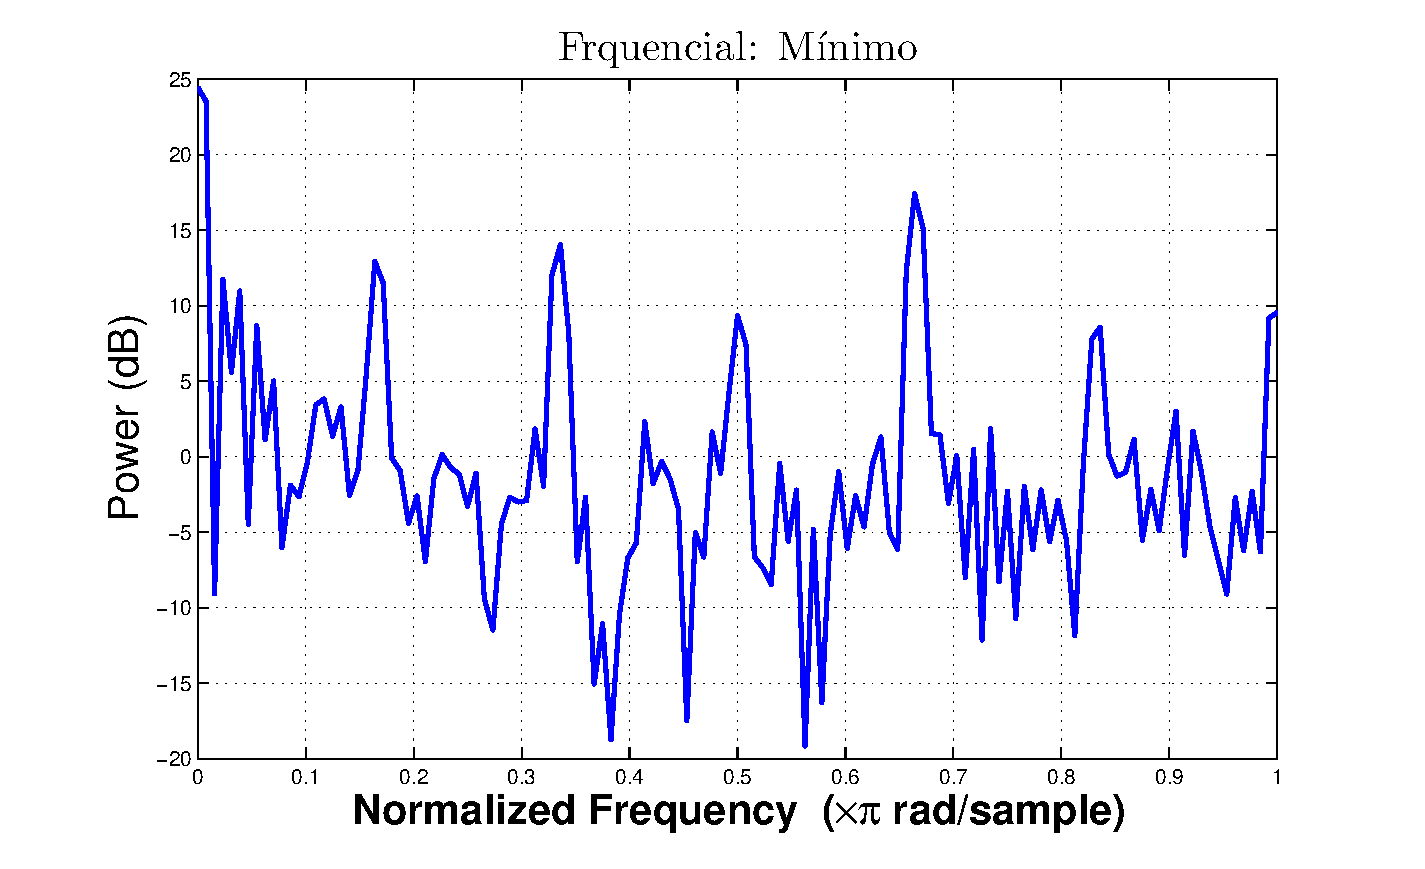
\includegraphics[width=0.9\columnwidth]{fq3}
\end{center}
\end{figure}
\end{frame}

\begin{frame}\frametitle{Análise: Visualização no domínio frequencial}
\begin{figure}[htpb] \begin{center} 
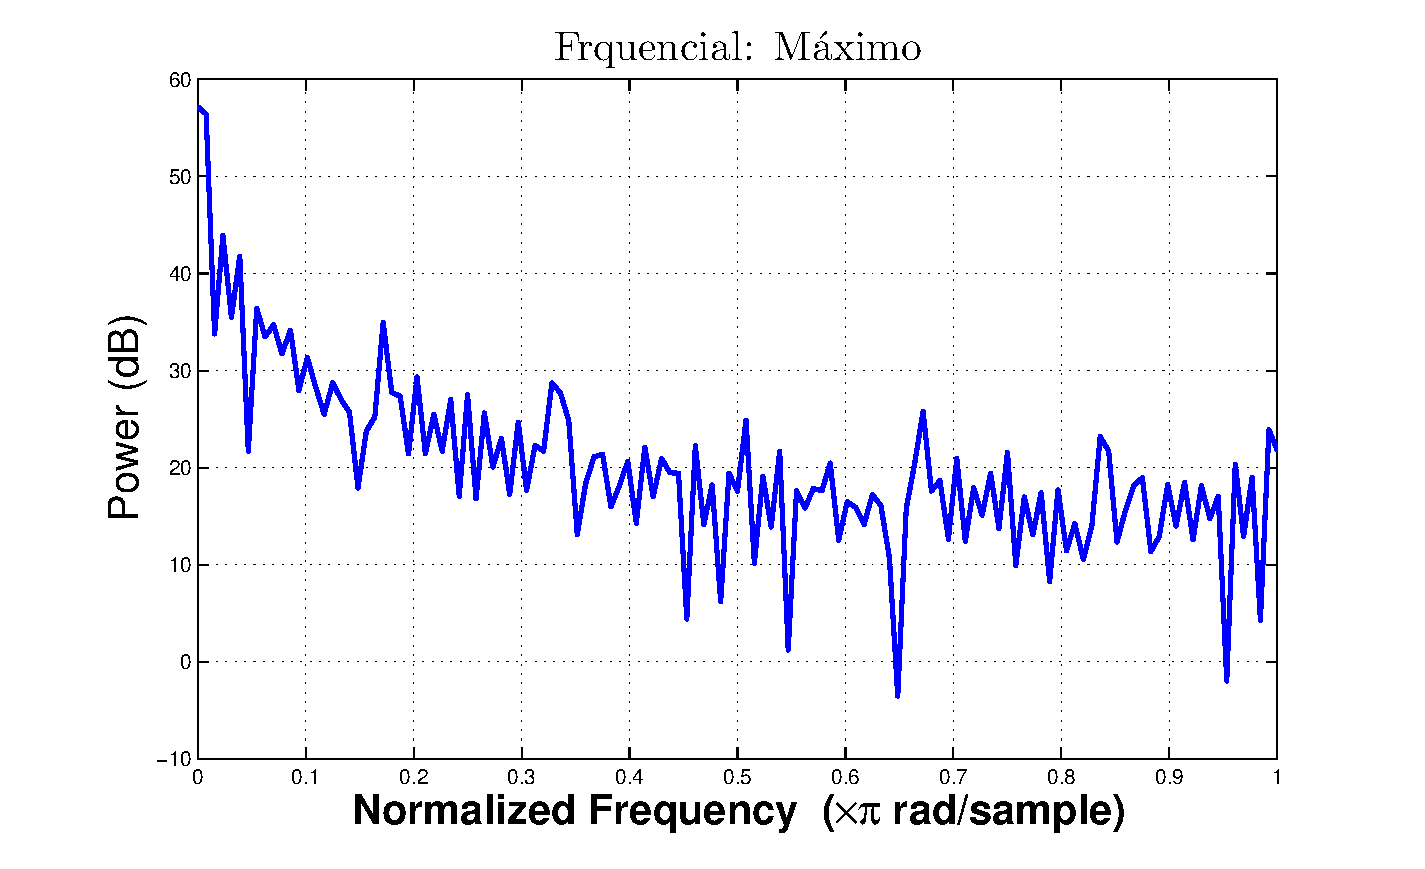
\includegraphics[width=0.9\columnwidth]{fq4}
\end{center}
\end{figure}
\end{frame}

\subsection{Histogramas}
\begin{frame}\frametitle{Análise: histogramas}

\begin{itemize}
\item Identificar grupo de valores que ao serem considerados podem causar distorções (\emph{bias}) na estimativa, diminuindo sua qualidade.
\item Conforme primeiras visualizações, o ano de 2013 apresenta valores médios atipicamente altos. Também se observa que os anos de 2012 e 2017 valores mais destoantes.
\item Os valores de médias mais altas aparecem de forma saliente nos histogramas e muito acima da curva gaussiana. Já os valores mais baixos, como os valores dos anos de 2016 e 2017 estão mais próximos da curva gaussiana. 
\end{itemize}

\end{frame}

\begin{frame}\frametitle{Análise: histogramas}
\begin{figure}[htpb] \begin{center} 
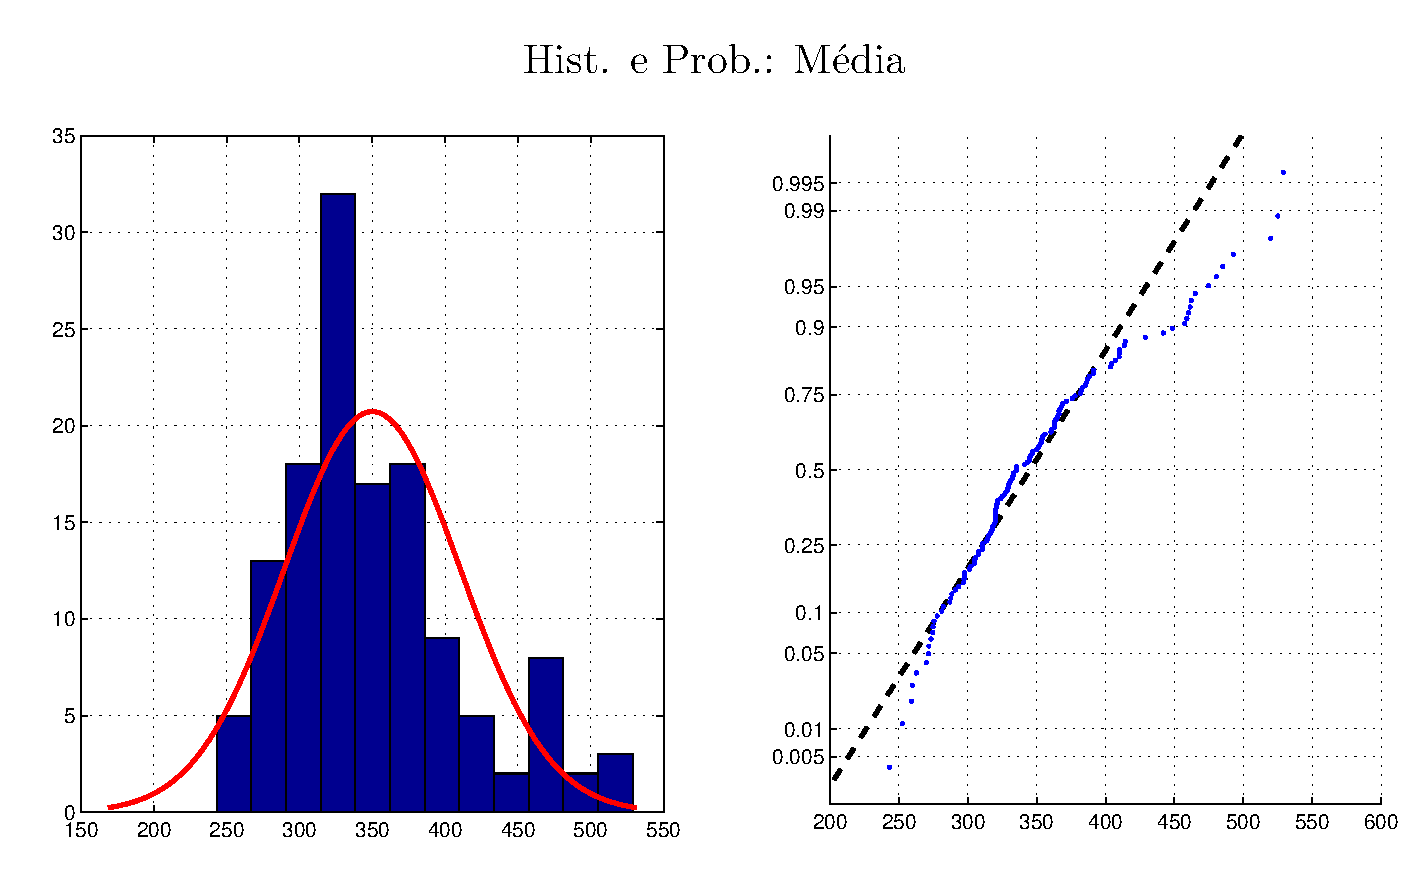
\includegraphics[width=0.9\columnwidth]{hist1}
\end{center}
\end{figure}
\end{frame}

\subsection{Conclusões}
\begin{frame}\frametitle{Análise: Conclusões}

\begin{itemize}
\item Não há padrões anuais dos quais pode-se valer para melhorar a estimativa.
\item O padrão mensal é significativo e pode ser usado para se obter uma melhor estimativa.
\item Reforçado pela análise frequencial, uma estimativa usando a média seria o mais indicado.
\item As amostras dos anos de 2012 e 2013 adicionam significativa distorção e quanto aos anos de 2016 e 2017 não.
\item Há uma relação de tendência nos pares 2012/2013 e 2016/2017.
\end{itemize}

\end{frame}

\section{Solução}
\subsection{Base teórica}
\begin{frame}\frametitle{Solução: base teórica}

Basicamente, pode-se utilizar a noção de valor esperado. Para o caso discreto, considerando o valor de alvo mensal como uma variável aleatória $X$, a esperança dessa variável é obtida com \cite{soderstrom1989system}:
\begin{equation}
E \left [ X \right ] = \Sum_{i=1}^N x_i p(x_i) = \mu_X
\end{equation}
\noindent sendo $x_i$ todos os $i$ valores possíveis e sua respectiva probabilidade $p(\cdot)$, e o valor médio $\mu_X$. Como o modelo utilizado é uma distribuição normal (gaussiana), a melhor expectativa para o valor de alvo mensal é dada pela média simples
\begin{equation}
\mu_X = \frac{1}{N} \Sum_{i=1}^N x_i 
\end{equation}
\noindent com o desvio padrão obtido com
\begin{equation}
\sigma_X = \sqrt{\frac{1}{N-1} \Sum_{i=1}^N \left ( x_i - \mu_X \right )^2}
\end{equation}

\end{frame}

\begin{frame}\frametitle{Solução: proposta}

\begin{itemize}
\item Como resposta ao desafio, calcula-se as médias mensais de todos os anos da série histórica, exceto dos meses dos anos 2012 e 2013, como uma estimativa para os meses de 2018. Sendo a estimativa desse ano a média das médias mensais.
\end{itemize}

\end{frame}

\subsection{Resultados}
\begin{frame}\frametitle{Solução: resultados}
\begin{figure}[htpb] \begin{center} 
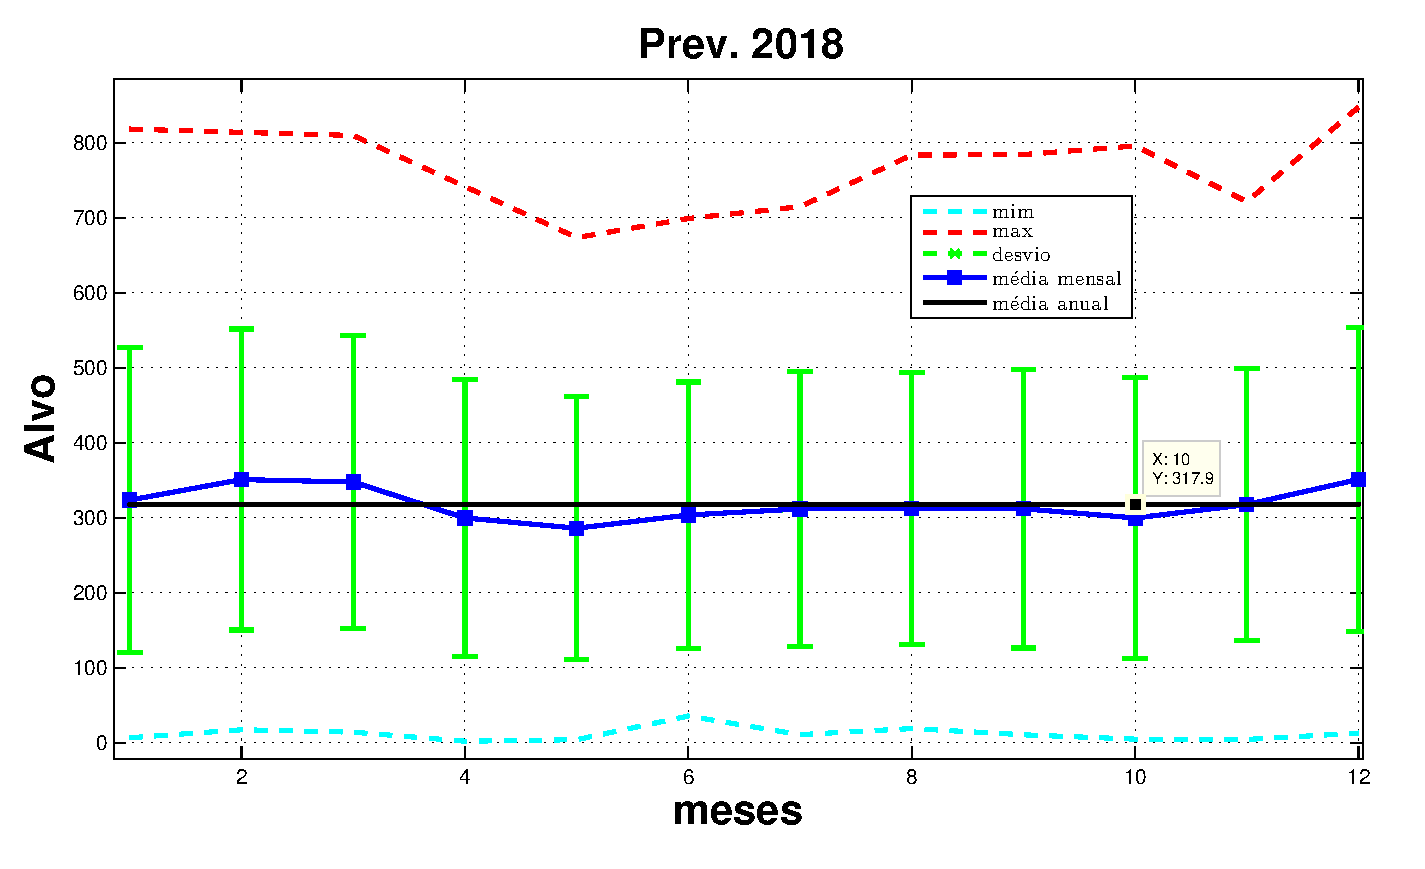
\includegraphics[width=0.9\columnwidth]{prev1}
\end{center}
\end{figure}
\end{frame}


\begin{frame}\frametitle{Solução: resultados}
\begin{figure}[htpb] \begin{center} 
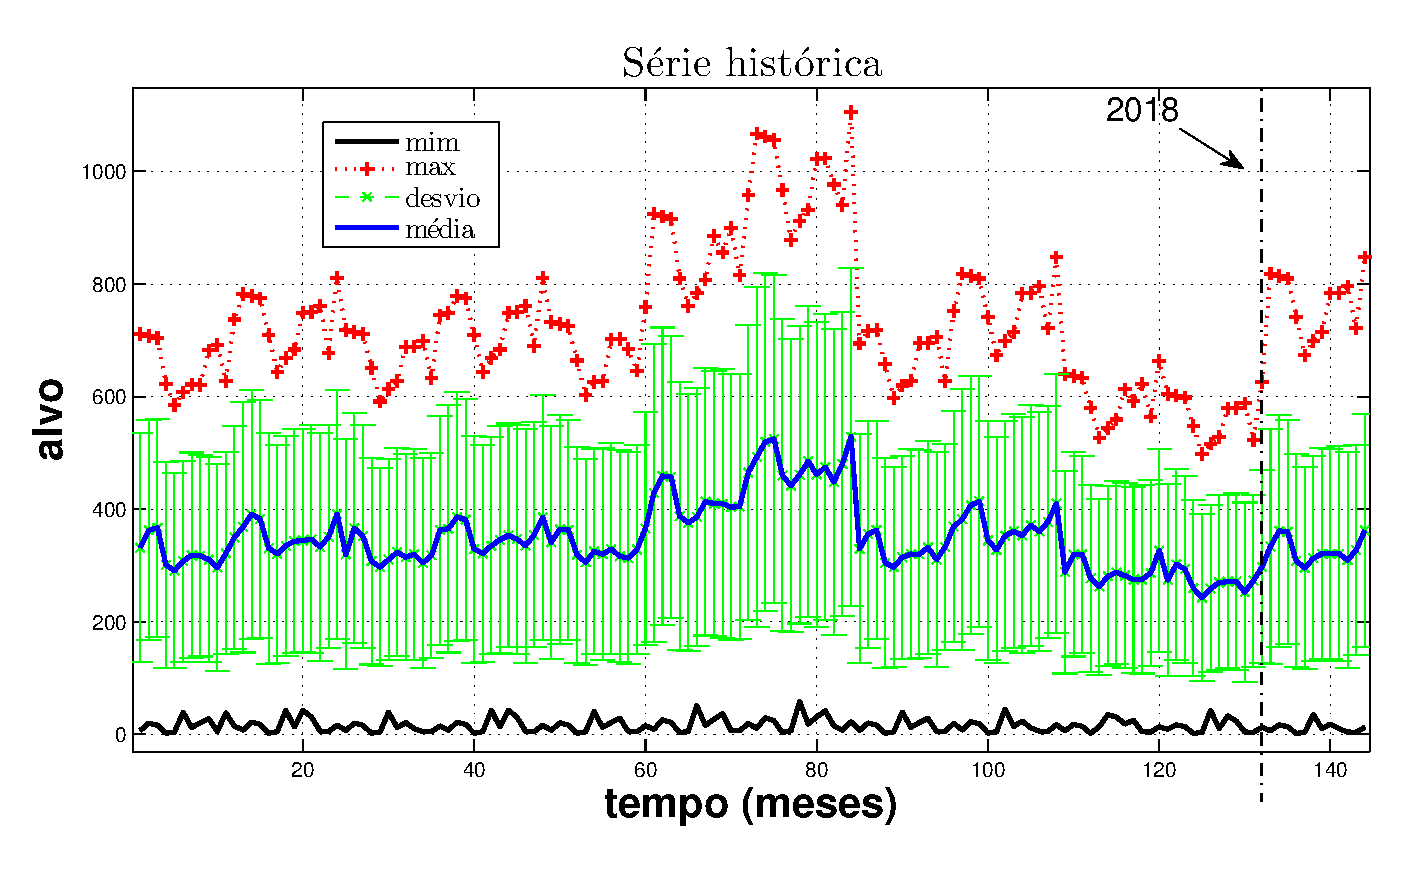
\includegraphics[width=0.9\columnwidth]{prev2}
\end{center}
\end{figure}
\end{frame}


\begin{frame}\frametitle{Solução: resultados}
\begin{figure}[htpb] \begin{center} 
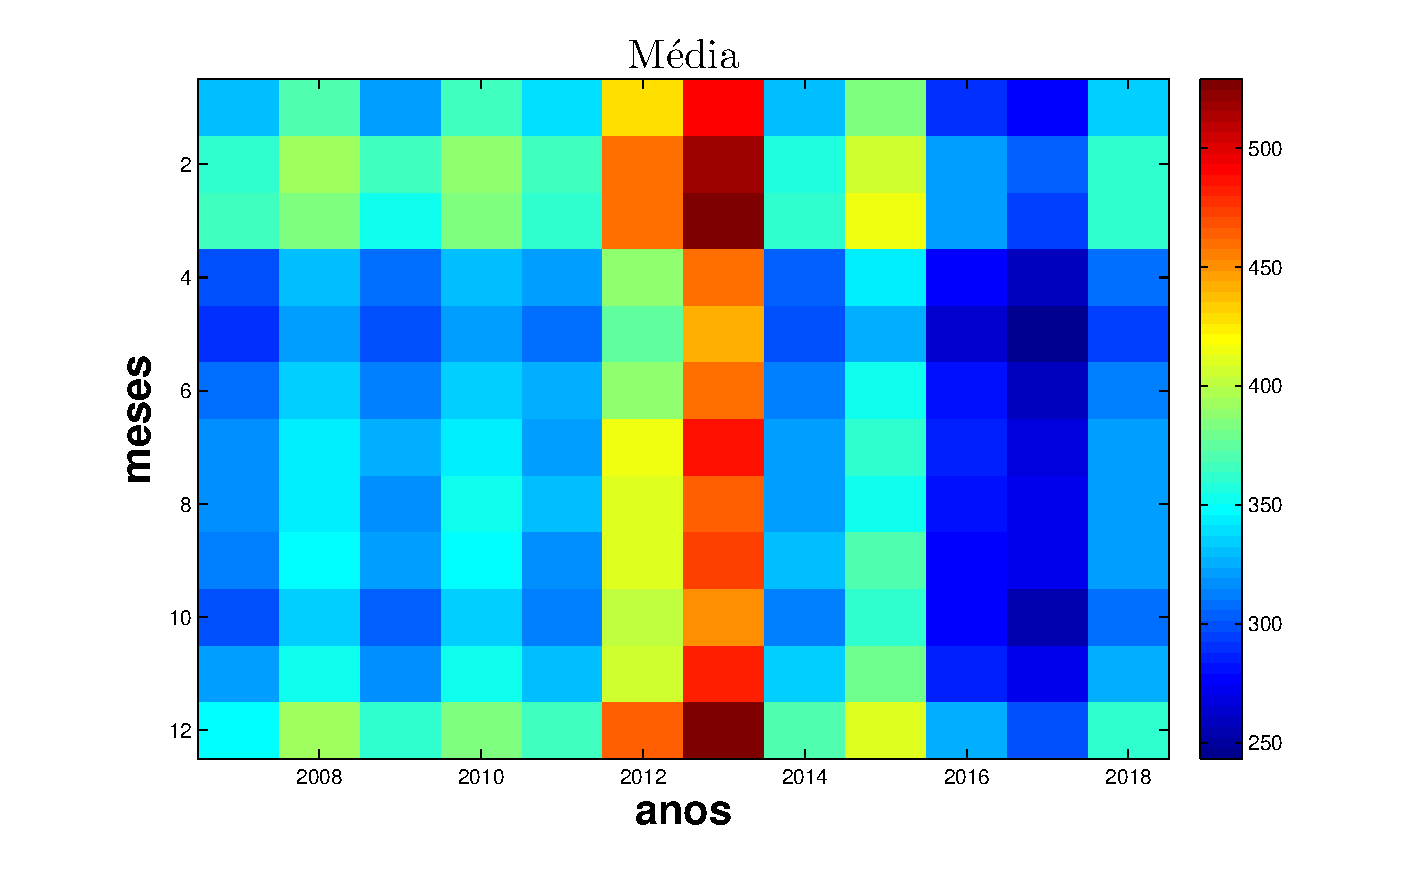
\includegraphics[width=0.9\columnwidth]{prev3}
\end{center}
\end{figure}
\end{frame}


\section{Conclusão}
\begin{frame}\frametitle{Conclusão}

\begin{itemize}
\item Considera-se como respondido o desafio frente a análise dos dados disponíveis, seguida de uma proposta de estimativa com embasamento teórico e em evidências técnicas.
\item Devido ao que foi exigido no desafio e pelo princípio da parcimônia, os dados referentes às variáveis não identificadas foram ignorados.
\end{itemize}

\end{frame}

\section{Notas}
\begin{frame}\frametitle{Notas}

\begin{itemize}
\item Poder-se-ia avaliar os histogramas mensais, evitando a análise frequencial, para se concluir que há um padrão mensal e esse pode ser modelado por uma distribuição normal. 
\item Numa análise de histograma das 20 variáveis não identificadas, observou-se na sua maioria uma distribuição gaussiana. Por meio de uma análises nos domínios temporal e frequencial, observou-se sinais altamente ruidosos. Também foi observado que 9 dessas variáveis apresenta valores dispares no ano de 2007. 
\item Quanto ao fato de 9 variáveis terem valores díspares apenas no ano de 2007 e os valores de Alvo não serem díspares, pode-se concluir que tais variáveis não afetam significativamente o valor Alvo.
\item Pode-se concluir, então, que o uso das variável não identificadas para a estimativa traria melhora não significativa ou até nula, não compensando o alto custo computacional e complexidade da aplicação para usá-las.
\end{itemize}

\end{frame}


\section*{Agradecimento}
\begin{frame}
Obrigado pela atenção e pela oportunidade.
\end{frame}

\bibliographystyle{IEEEtran}
% \bibliographystyle{abntex2-alf} 
%\bibliographystyle{unsrtnat}
\bibliography{Robotics,computacao,referencias}

\end{document}


